\section{Brikker}

Formålet med at implementere brikker i spillet var at give gameplayet en helt ny dimension. 

\begin{itemize}
\item \textbf{Tegne Brikker.} For lettest at kunne holde styr på brikkerne har vi lavet en struct, \texttt{Brick} der repræsenterer en brik. Den indeholder position i x- og y-koordinater, bredde, højde og brikkens liv. Brikkerne i en bane er gemt i et array:\\ \texttt{Brick bricks[BRICK\_TABLE\_HEIGHT][BRICK\_TABLE\_WIDTH];}. Når banen initialiseres gennemløbes dette array og hver brik tildeles koordinater, bredde, højde og liv. Efter dette tegnes brikken. Hvis brikken har 0 liv svarer det til at der ikke er en brik. Ved at give brikkerne i array'et forskellige antal liv kan man lave mønstre med brikkerne så man på den måde har flere forskellige baner i spillet. På Figur \ref{fig:brikker} er der vist hvordan brikker med forskelligt antal liv er tegnet. Jo flere liv de har, des mere solide tegnes de. Som et lille twist i gameplayet har vi valgt at gøre brikker med mere end fem liv usynlige så de pludseligt kan dukke op når man rammer dem. 
\begin{figure}[h!]
\centering
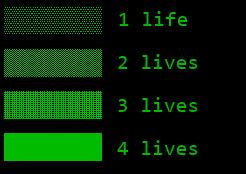
\includegraphics[scale=1]{figs/brikker.png}
\caption{Brikker med forskelligt antal liv tegnes forskelligt}
\label{fig:brikker}
\end{figure}
%\begin{itemize}
\item \textbf{Baner gemt i et array i ROM'en.} Vi har valgt at hardcode brikkernes bredde og højde for at spare plads når vi gemmer banerne i ROM'en. På denne måde kan en bane i ROM'en gemmes i arrayet\\ \texttt{unsigned char rom levels[6][BRICK\_TABLE\_HEIGHT][BRICK\_TABLE\_WIDTH]}. Dette arrray er et tredimensionalt array af chars der er gemt i ROM'en. Det indeholder 6 "lag" der hver indeholder de todimensionale data til en bane. Værdien af hver char er antallet af liv den tilsvarende brik får. Når banen initialiseres, løbes dette array og arrayet \texttt{bricks[BRICK\_TABLE\_HEIGHT][BRICK\_TABLE\_WIDTH]} igennem og brikkerne i \texttt{bricks} får det antal liv der står i \texttt{levels} arrayet. Den dynamiske hukommelse i mikroprocessoren indeholder således kun et array af brikker der svarer til den aktuelle bane. Et eksempel på hvordan en bane er gemt i arrayet \texttt{levels} er vist nedenfor.
\begin{lstlisting}[frame=single]
{
    { 0, 0, 0, 0, 0, 0, 0, 0, 0, 0, 0, 0, 0, 0 },
    { 0, 0, 0, 0, 0, 0, 0, 0, 0, 0, 0, 0, 0, 0 },
    { 0, 0, 0, 0, 0, 0, 0, 0, 0, 0, 0, 0, 0, 0 },
    { 0, 0, 0, 0, 0, 0, 0, 0, 0, 0, 0, 0, 0, 0 },
    { 0, 0, 0, 0, 0, 0, 0, 0, 0, 0, 0, 0, 0, 0 },
    { 0, 0, 0, 0, 0, 0, 0, 0, 0, 0, 0, 0, 0, 0 },
    { 0, 1, 1, 1, 1, 1, 1, 1, 1, 1, 1, 1, 1, 0 },
    { 0, 1, 1, 1, 1, 1, 1, 1, 1, 1, 1, 1, 1, 0 },
    { 0, 2, 2, 2, 2, 2, 2, 2, 2, 2, 2, 2, 2, 0 },
    { 0, 3, 3, 3, 3, 3, 3, 3, 3, 3, 3, 3, 3, 0 },
    { 0, 4, 4, 4, 4, 4, 4, 4, 4, 4, 4, 4, 4, 0 },
    { 0, 0, 0, 0, 0, 0, 0, 0, 0, 0, 0, 0, 0, 0 },
    { 0, 0, 0, 0, 0, 0, 0, 0, 0, 0, 0, 0, 0, 0 },
    { 0, 0, 0, 0, 0, 0, 0, 0, 0, 0, 0, 0, 0, 0 },
    { 0, 0, 0, 0, 0, 0, 0, 0, 0, 0, 0, 0, 0, 0 },
    { 0, 0, 0, 0, 0, 0, 0, 0, 0, 0, 0, 0, 0, 0 },
    { 0, 0, 0, 0, 0, 0, 0, 0, 0, 0, 0, 0, 0, 0 },
    { 0, 0, 0, 0, 0, 0, 0, 0, 0, 0, 0, 0, 0, 0 },
    { 0, 0, 0, 0, 0, 0, 0, 0, 0, 0, 0, 0, 0, 0 },
},
\end{lstlisting}
Banen der svarer til det ovenstående array, er vist på Figur \ref{fig:level1}. 

\begin{figure}[h!]
\centering
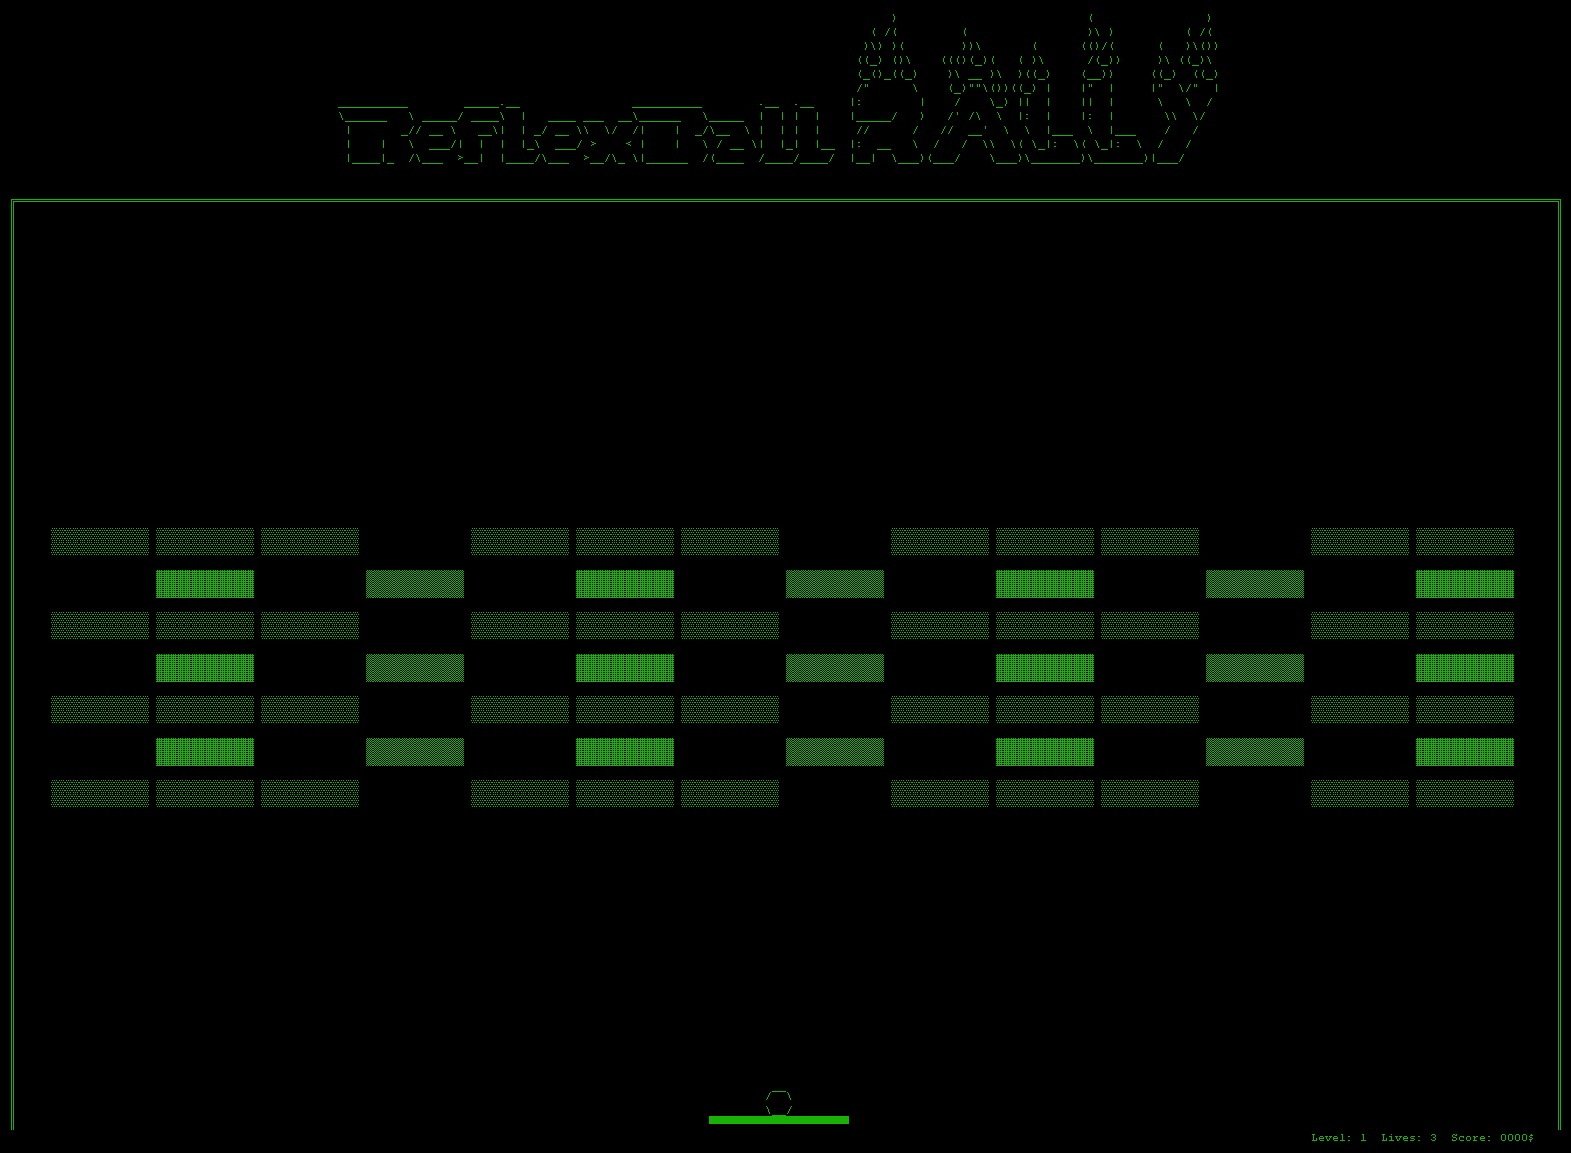
\includegraphics[scale=0.25]{figs/screenshots/level1.png}
\caption{Level 1 i spillet}
\label{fig:level1}
\end{figure}

%\end{itemize}
\item \textbf{Tjekke om man rammer brikker.} Den helt store udfordring med brikkerne var at tjekke om bolden ramte dem. Ved hver eneste iteration af spillet gennemløber vi arrayet \texttt{bricks[][]} og for alle brikker med mere end 0 liv tjekker vi om bolden har ramt og i givet fald hvordan.\\
Når spillet itereres og bolden flyttes tjekker vi først om bolden rammer brikkerne før vi tegner den. Hvis bolden har ramt en brik reflekteres den og får sin nye position før den tegnes. Hvis bolden har ramt en brik, er boldens koordinater altså inde i brikken når vi tjekker.

For at bolden skulle bevæge sig lige hurtigt i begge retninger på skærmen har vi lavet x-komposanten af boldens vektor dobbelt så stor. Det giver nogle ekstra udfordringer når bolden rammer brikkerne. Når bolden kan bevæge sig 2 karakterer i x-retningen kan den ramme brikkerne fra siden på en række forskellige måder. Disse er vist for højre side af brikken på Figur \ref{fig:SideReflexSamlet}. 
Når vi har itereret spillet og tjekker boldens position kan den på x-aksen befinde sig både en eller to karakterer inde i brikken. Den kan således ramme brikken på seks forskellige måder som vist på ovennævnte figur. Det er vigtigt at tage højde for at bolden kan ramme to karakterer ind i brikken når man tjekker om bolden har ramt brikken for siden i midten. Hvis man ikke tager højde for dette, vil bolden bevæge sig igennem brikken mens den reflekteres af toppe og bunden. 

\begin{figure}[h!]
\centering
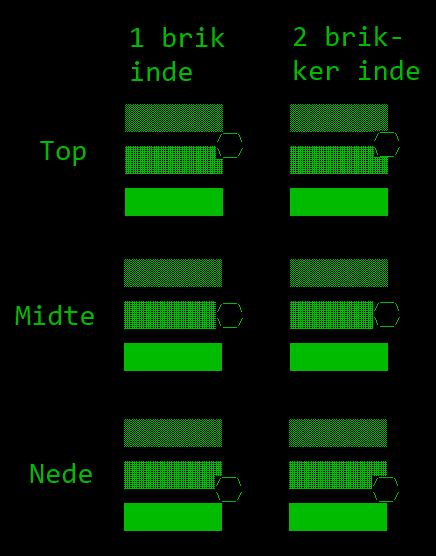
\includegraphics[scale=0.75]{figs/side_reflex_samlet.png}
\caption{Forskellige måder bolden kan ramme fra siden}
\label{fig:SideReflexSamlet}
\end{figure}


For at give et godt gameplay har vi besluttet at bolden fortrinsvis skal reflekteres ned og op så brugeren kan få den. Dette er vist på Figur \ref{fig:ReflexOppeFri}. Når bolden rammer brikken fra toppen og er 2 karakterer inde i brikken vil den blive reflekteret som vist på figuren. Hvis bolden havde ramt på samme måde, men var kommet nedefra var den blevet reflekteret som om den havde ramt siden af brikken.

Det der er vist på denne figur er, borset fra de omgivende brikker, samme situation som på Figur \ref{fig:SideReflexSamlet}, Top, 2 brikker inde. 

 
\begin{figure}[h!]
\centering
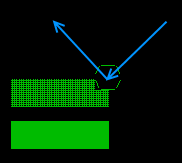
\includegraphics[scale=1]{figs/reflex_oppe_fri.png}
\caption{Forskellige måder bolden kan ramme fra siden}
\label{fig:ReflexOppeFri}
\end{figure}



\begin{itemize}
\item Højre/venstre og oppe/nede
\item Kanter?
\end{itemize}
\item Trække liv fra brikkerne
\item Lave deflect på baggrund af om der er brikker omkring brikken
\begin{itemize}
\item Forklare tilfældene med at ramme to brikker af gangen
\item Forklare tilfældene med at ramme flere hjørner
\end{itemize}
\item Briklogik korrigeret fordi der bevæges 2 karakterer i x-retningen
\end{itemize}

\subsection{Flowchart for briklogikken}

\newpage

% Flowcharting techniques for easy maintenance
% Author: Brent Longborough
% =================================================
% Set up a few colours
%\colorlet{lcfree}{Green3}
%\colorlet{lcnorm}{Blue3}
%\colorlet{lccong}{Red3}
% -------------------------------------------------
% Set up a new layer for the debugging marks, and make sure it is on
% top
\pgfdeclarelayer{marx}
\pgfsetlayers{main,marx}
% A macro for marking coordinates (specific to the coordinate naming
% scheme used here). Swap the following 2 definitions to deactivate
% marks.
\providecommand{\cmark}[2][]{%
  \begin{pgfonlayer}{marx}
    \node [nmark] at (c#2#1) {#2};
  \end{pgfonlayer}{marx}
  } 
\providecommand{\cmark}[2][]{\relax} 
% -------------------------------------------------
% Start the picture
\begin{center}
\newgeometry{margin=1cm}
\begin{tikzpicture}[%
    >=triangle 60,              % Nice arrows; your taste may be different
    start chain=going below,    % General flow is top-to-bottom
    node distance=4mm and 40mm, % Global setup of box spacing
    every join/.style={norm},   % Default linetype for connecting boxes
    ]
% ------------------------------------------------- 
% A few box styles 

% <on chain> *and* <on grid> reduce the need for manual relative
% positioning of nodes
\tikzset{
  base/.style={draw, on chain, on grid, align=center, minimum height=2ex},
  proc/.style={base, rectangle, fill=blue!30, font={\tiny}},
  test/.style={base, diamond, aspect=2.2, fill=orange!40, font={\tiny}},
  term/.style={proc, rounded corners,fill=green!30, font={\tiny}},
  placeholder/.style={base, on chain, text width=6em, fill=white, font={\tiny}},
  % coord node style is used for placing corners of connecting lines
  coord/.style={coordinate, on chain, on grid, node distance=4mm and 4mm},
  % nmark node style is used for coordinate debugging marks
  nmark/.style={draw, cyan, circle, font={\sffamily\bfseries}},
  % -------------------------------------------------
  % Connector line styles for different parts of the diagram
  norm/.style={->, draw},
  free/.style={->, draw},
  cong/.style={->, draw},
  it/.style={font={\tiny}}
}
% -------------------------------------------------
% Start by placing the nodes
\node [proc, it] (p0) {Iterate ball};
\node [test, join] (t0) {Indenfor bane?};

% No join for exits from test nodes - connections have more complex
% requirements
% We continue until all the blocks are positioned
\node [proc, fill=gray!30] (p1) {For(alle brikker)};
\node [test, join]	(t1)	{Ramt brik?};
\node [term]    	(p2) 	{score++};
\node [test, join]	(t2) 	{Top/bund?};
\node [test] 		(t3)	{DeflectedY?};
\node [test] 		(t4) 	{Top, ven- \\ stre/højre?};
\node [test] 		(t5)	{Brik over?};
\node [term]  		(p3)    {dontDeflectY};

\node [placeholder, opacity=0] {};
\node [placeholder, opacity=0] {};
\node [placeholder, opacity=0] {};
\node [placeholder, opacity=0] {};
\node [placeholder, opacity=0] {};

\node [test]		(t8)  {Ramt midt \\ i brikken?};
\node [term]  		(p5)  {dontDeflectY};
\node [test, join]	(t9)  {Top fra neden?};
\node [term]		(p6)	  {dontDeflectY};


\node [test, join]	(t11)		{dontDeflectY?};
\node [proc, it] 	(p8) 		{Reflekter Y};


% We position the next block explicitly as the first block in the
% second column.  The chain 'comes along with us'. The distance
% between columns has already been defined, so we don't need to
% specify it.
%%%% NÆSTE KOLONNE
\node [placeholder, opacity=0, right=of t0] (k0) {};


\node [placeholder, opacity=0, right=of t4]  {};
\node [test] 	(t6) {Bund, ven- \\ stre/højre?};
\node [test]				(t7) {Brik under?};
\node [term]      	  		(p4) {dontDeflectY};

\node [test, right=of t9] 	(t10)  	{Bund fra oven?};
\node [term]      			(p7)	{dontDeflectY};


%%%% NÆSTE KOLONNE
\node [placeholder, opacity=0, right=of k0]  {};
\node [test] 	(t12) {Side? \& !xDeflected};
\node [test] 				(t13) {Top/bund?};
\node [test] 				(t14) {Venstre \& \\ brik til venstre?};
%\node [test] (t14) {Levende brik til venstre?};
\node [term] 				(p9)  {dontDeflectX};
\node [test, join] 			(t15) {Højre side \& \\ brik til højre?};
%\node [test] (t16) {Levende brik til højre?};
\node [term]      			(p10)  {dontDeflectX};

\node [placeholder, opacity=0]  (k3) {};
\node [test, join] 	(t16) {Venstre side?};
\node [test] 		(t17) {Kommer fra \\ højre?};
\node [term]      	(p11) {dontDeflectX};
% Tre til højre for som er under i hieraki

\node [placeholder, opacity=0]  {};
\node [test] 	(t20) {Fra siden, \\ ml. top \\ og bund?};
\node [test] 		(t21) {Top?};
\node [test] 		(t22) {Fra oven \& \\ frit over?};
\node [term]      	(p13) {dontDeflectX};
\node [test, join] 	(t24) {dontDeflectX?};
\node [proc, it] 	(p15) {Reflekter X};


%%\node [test] (t19) {Højre side?};
%%%%% NÆSTE KOLONNE
\node [placeholder, opacity=0, right=of t12] (k1) {};
\node [test, right=of t16] 	(t18) {Højre side?};
\node [test] 				(t19) {Kommer fra \\ venstre?};
\node [term]      			(p12) {dontDeflectX};

\node [test, right=of t22] 	(t23) {Fra neden \& \\ frit under?};
\node [term]    			(p14) {dontDeflectX};

%%%%% NÆSTE KOLONNE
\node [test, right=of k1] 	(t25) {Under striker?};
\node [test] 				(t26) {gameStarted?};
\node [test] 				(t27) {Udenfor sider?};
\node [proc, it] 			(p16) {Reflekter X};
\node [test, join]			(t28) {Over top/ \\ på striker?};
\node [test] 				(t29) {Ramt striker?};
\node [proc] 				(p17) {Roter afhængigt \\ af hvor man rammer};
\node [proc, join] 			(p18) {Reflekter Y};
\node [proc, join] 			(p19) {drawBigBall};






% -------------------------------------------------
% Now we place the coordinate nodes for the connectors with angles, or
% with annotations. We also mark them for debugging.
%\node [coord, right=of t1] (c1)  {}; %\cmark{1}   
%\node [coord, right=of t3] (c3)  {}; %\cmark{3}   
%\node [coord, right=of t6] (c6)  {}; %\cmark{6}   
%\node [coord, right=of t7] (c7)  {}; %\cmark{7}   
%\node [coord, left=of t4]  (c4)  {}; %\cmark{4}   
%\node [coord, right=of t4] (c4r) {}; %\cmark[r]{4}
%\node [coord, left=of t7]  (c5)  {}; %\cmark{5} 

% -------------------------------------------------

% -------------------------------------------------
% All the other connections come out of tests and need annotating
% First, the straight north-south connections. In each case, we first
% draw a path with a (consistently positioned) annotation node, then
% we draw the arrow itself.
\path (t0.south) to node [near start, xshift=1em] {$ja$} (p1);
  \draw [->] (t0.south) -- (p1);
 
\path (t1.south) to node [near start, xshift=1em] {$ja$} (p2);
  \draw [->] (t1.south) -- (p2);
  
\path (t2.south) to node [near start, xshift=1em] {$ja$} (t3);
  \draw [->] (t2.south) -- (t3);  

\path (t3.south) to node [near start, xshift=1em] {$nej$} (t4);
  \draw [->] (t3.south) -- (t4);
  
\path (t4.south) to node [near start, xshift=1em] {$ja$} (t5);
  \draw [->] (t4.south) -- (t5);

\path (t5.south) to node [near start, xshift=1em] {$ja$} (p3);
  \draw [->] (t5.south) -- (p3); 

\path (t8.south) to node [near start, xshift=1em] {$ja$} (p5);
  \draw [->] (t8.south) -- (p5);
  
\path (t9.south) to node [near start, xshift=1em] {$ja$} (p6);
  \draw [->] (t9.south) -- (p6); 
  
\path (t11.south) to node [near start, xshift=1em] {$nej$} (p8);
  \draw [->] (t11.south) -- (p8);
  
%%Næste række (mellemrække)
\path (t6.south) to node [near start, xshift=1em] {$ja$} (t7);
  \draw [->] (t6.south) -- (t7);
 
\path (t7.south) to node [near start, xshift=1em] {$ja$} (p4);
  \draw [->] (t7.south) -- (p4);
  
\path (t10.south) to node [near start, xshift=1em] {$ja$} (p7);
  \draw [->] (t10.south) -- (p7);

%%Næste række
\path (t12.south) to node [near start, xshift=1em] {$ja$} (t13);
  \draw [->] (t12.south) -- (t13); 
  
\path (t13.south) to node [near start, xshift=1em] {$ja$} (t14);
  \draw [->] (t13.south) -- (t14);

\path (t14.south) to node [near start, xshift=1em] {$ja$} (p9);
  \draw [->] (t14.south) -- (p9); 

\path (t15.south) to node [near start, xshift=1em] {$ja$} (p10);
  \draw [->] (t15.south) -- (p10); 

\path (t16.south) to node [near start, xshift=1em] {$ja$} (t17);
  \draw [->] (t16.south) -- (t17); 

\path (t17.south) to node [near start, xshift=1em] {$ja$} (p11);
  \draw [->] (t17.south) -- (p11);

\path (t20.south) to node [near start, xshift=1em] {$ja$} (t21);
  \draw [->] (t20.south) -- (t21);
  
\path (t21.south) to node [near start, xshift=1em] {$ja$} (t22);
  \draw [->] (t21.south) -- (t22);  

\path (t22.south) to node [near start, xshift=1em] {$ja$} (p13);
  \draw [->] (t22.south) -- (p13);

\path (t24.south) to node [near start, xshift=1em] {$nej$} (p15);
  \draw [->] (t24.south) -- (p15);
  

% Næste række (mellemrække)
\path (t18.south) to node [near start, xshift=1em] {$ja$} (t19);
  \draw [->] (t18.south) -- (t19);

\path (t19.south) to node [near start, xshift=1em] {$ja$} (p12);
  \draw [->] (t19.south) -- (p12);

\path (t23.south) to node [near start, xshift=1em] {$ja$} (p14);
  \draw [->] (t23.south) -- (p14);


% Næste række
\path (t25.south) to node [near start, xshift=1em] {$nej$} (t26);
  \draw [->] (t25.south) -- (t26);

\path (t26.south) to node [near start, xshift=1em] {$ja$} (t27);
  \draw [->] (t26.south) -- (t27);
  
\path (t27.south) to node [near start, xshift=1em] {$ja$} (p16);
  \draw [->] (t27.south) -- (p16);
  
\path (t28.south) to node [near start, xshift=1em] {$ja$} (t29);
  \draw [->] (t28.south) -- (t29);
  
\path (t29.south) to node [near start, xshift=1em] {$ja$} (p17);
  \draw [->] (t29.south) -- (p17);




%\path (t6.south) to node [near start, xshift=1em] {$y$} (t7); 
% \draw [*->,lcfree] (t6.south) -- (t7); 
% ------------------------------------------------- 
% Now the straight east-west connections. To provide consistent
% positioning of the test exit annotations, we have positioned
% coordinates for the vertical part of the connectors. The annotation
% text is positioned on a path to the coordinate, and then the whole
% connector is drawn to its destination box.
%\path (t3.east) to node [near start, yshift=1em] {$n$} (c3); 
%  \draw [o->,lccong] (t3.east) -- (p8);
%\path (t4.east) to node [yshift=-1em] {$k \leq 0$} (c4r); 
%  \draw [o->,lcnorm] (t4.east) -- (p9);

% -------------------------------------------------
% The coordinates

\node [coord, right = 20mm of p1] (cp1)  {}; %\cmark{1}
\node [coord, right = 20mm of t1] (ct1)  {}; %\cmark{1}
\node [coord, right = 20mm of t4] (ct4)  {}; %\cmark{1} 
\node [coord, below = of p3] (cp3)  {}; %\cmark{1}
\node [coord, right = 20mm of t5] (ct5)  {}; %\cmark{1}

\node [coord, right = 18mm of t8] (ct8)  {}; %\cmark{1}
\node [coord, below = of p5] (cp5)  {}; %\cmark{1}
\node [coord, right = 22mm of p5] (cp5r)  {}; %\cmark{1}
\node [coord, right = 22mm of t9] (ct9)  {}; %\cmark{1}

\node [coord, right = 22mm of t11] (ct11)  {}; %\cmark{1}
\node [coord, below = 20 mm of ct11] (cp8)  {}; %\cmark{1}
\node [coord, right = 40 mm of cp8] (cp8r)  {}; %\cmark{1}



% Næste kolonne (mellemrække)
\node [coord, below = of p4] (cp4)  {}; %\cmark{1}
\node [coord, right = 20mm of t6] (ct6)  {}; %\cmark{1}
\node [coord, right = 20mm of t7] (ct7)  {}; %\cmark{1}
\node [coord, right = 18mm of t10] (ct10)  {}; %\cmark{1}
\node [coord, below = of p7] (cp7)  {}; %\cmark{1}


% Næste kolonne
\node [coord, right = 62 mm of t0] (ct12)  {}; %\cmark{1}
\node [coord, right = 62 mm of t2] (ct2r)  {}; %\cmark{1}
\node [coord, right = 62 mm of t3] (ct3r)  {}; %\cmark{1}


\node [coord, right = 23 mm of t13] (ct13)  {}; %\cmark{1}


\node [coord, right = 20 mm of t14] (ct14)  {}; %\cmark{1}
\node [coord, below = of p9] (cp9)  {}; %\cmark{1}

\node [coord, right = 20 mm of t15] (ct15)  {}; %\cmark{1}
\node [coord, below = of p10] (cp10)  {}; %\cmark{1}
\node [coord, right = 20 mm of cp10] (cp10r)  {}; %\cmark{1}

\node [coord, below = of p11] (cp11)  {}; %\cmark{1}
\node [coord, below = of cp11] (cp11b)  {}; %\cmark{1}

\node [coord, below = of k3] (ck3b)  {}; %\cmark{1}
\node [coord, right = 22 mm of ck3b] (ck3)  {}; %\cmark{1}
\node [coord, right = 22 mm of t16] (ct16)  {}; %\cmark{1}
\node [coord, right = 22 mm of t17] (ct17)  {}; %\cmark{1}

\node [coord, right = 20 mm of t18] (ct18)  {}; %\cmark{1}
\node [coord, right = 20 mm of t19] (ct19)  {}; %\cmark{1}

\node [coord, below = of p13] (cp13)  {}; %\cmark{1}
\node [coord, right = 21 mm of cp13] (cp13r)  {}; %\cmark{1}

\node [coord, below = of p14] (cp14)  {}; %\cmark{1}


% -------------------------------------------------
% Finally, the twisty connectors. Again, we place the annotation
% first, then draw the connector

% Næste kolonne 

\path (t14.east) to node [very near start, yshift=1em] {$nej$} (ct14); 
  \draw [->] (t14.east) -- (ct14) |-(cp9) -| (t15);
  
\path (t15.east) to node [very near start, yshift=1em] {$nej$} (ct15); 
  \draw [->] (t15.east) -- (ct15) |-(cp10) -| (t16);
  
\path (t13.east) to node [very near start, yshift=1em] {$nej$} (ct13); 
  \draw [->] (t13.east) -- (ct13) |-(cp10r) ;

\path (p11.south) to node [very near start, yshift=1em] {} (cp11); 
  \draw [->] (p11.south) |- (cp11) -|(ck3) -| (t18) ;
  
\path (t16.east) to node [very near start, yshift=1em] {$nej$} (ct16); 
  \draw [->] (t16.east) -- (ct16);

\path (t17.east) to node [very near start, yshift=1em] {$nej$} (ct17); 
  \draw [->] (t17.east) -- (ct17);


\path (p12.south) to node [near start, yshift=1em] {} (cp11b); 
  \draw [->] (p12.south) |- (cp11b) -| (t20);
  
\path (t18.east) to node [very near start, yshift=1em] {$nej$} (ct18); 
  \draw [->] (t18.east) -| (ct18) |- (cp11b) -|(t20) ; 

\path (t19.east) to node [very near start, yshift=1em] {$nej$} (ct19); 
  \draw [->] (t19.east) -- (ct19) ; 

\path (t21.east) to node [very near start, yshift=1em] {$nej$} (t23); 
  \draw [->] (t21.east) -| (t23) ; 
  
\path (t22.east) to node [very near start, yshift=1em] {$nej$} (cp13r); 
  \draw [->] (t22.east) -| (cp13r) ; 

%% Slut nedenfor er starten


\path (t1.east) to node [very near start, yshift=1em] {$nej$} (ct1); 
  \draw [->] (t1.east) -| (cp1) --(p1);
  
\path (t2.east) to node [very near start, yshift=1em] {$nej$} (ct2r); 
  \draw [->] (t2.east) -- (ct2r);

\path (t3.east) to node [very near start, yshift=1em] {$nej$} (ct3r); 
  \draw [->] (t3.east) -- (ct3r); 
  
\path (t4.east) to node [very near start, yshift=1em] {$nej$} (t6); 
  \draw [->] (t4.east) -| (t6);

\path (p3.south) to node [very near start, yshift=1em] {} (cp3); 
  \draw [->] (p3.south) |- (cp3) -| (ct4);

\path (t5.east) to node [very near start, yshift=1em] {$nej$} (ct5); 
  \draw [->] (t5.east) -- (ct5);

\path (t8.east) to node [very near start, yshift=1em] {$nej$} (ct8); 
  \draw [->] (t8.east) -| (ct8) |- (cp5) -| (t9);

\path (t9.east) to node [very near start, yshift=1em] {$nej$} (ct9); 
  \draw [->] (t9.east) -| (ct9) |- (cp5r) -| (t10) ;

\path (t11.east) to node [very near start, yshift=1em] {$nej$} (ct11); 
  \draw [->] (t11.east) -- (ct11) -| (cp8); 
  
\path (p8.south) to node [very near start, yshift=1em] {} (cp8); 
  \draw [->] (p8.south) |- (cp8) -- (cp8r) |- (ct12) -| (t12); 


  
  
  
% Næste kolonne (mellemkolonne)  
\path (p4.south) to node [very near start, yshift=1em] {} (cp4); 
  \draw [->] (p4.south) -| (cp4) -| (t8);
  
\path (t6.east) to node [very near start, yshift=1em] {$nej$} (ct6); 
  \draw [->] (t6.east) -| (ct6) |- (cp4);

\path (t7.east) to node [very near start, yshift=1em] {$nej$} (ct7); 
  \draw [->] (t7.east) -- (ct7);
  
\path (t7.east) to node [very near start, yshift=1em] {$nej$} (ct7); 
  \draw [->] (t7.east) -- (ct7);

\path (p7.south) to node [very near start, yshift=1em] {} (cp7); 
  \draw [->] (p7.south) |- (cp7) -| (t11);

\path (t10.east) to node [very near start, yshift=1em] {$nej$} (ct10); 
  \draw [->] (t10.east) -| (ct10) |- (cp7);
  
  


%\path (t1.east) to node [near start, yshift=1em] {$n$} (c1); 
%  \draw [o->,lcfree] (t1.east) -- (c1) |- (p4);
%\path (t2.east) -| node [very near start, yshift=1em] {$n$} (c1); 
%  \draw [o->,lcfree] (t2.east) -| (c1);
%\path (t4.west) to node [yshift=-1em] {$k>0$} (c4); 
%  \draw [*->,lcnorm] (t4.west) -- (c4) |- (p3);
%\path (t5.east) -| node [very near start, yshift=1em] {$n$} (c6); 
%  \draw [o->,lcfree] (t5.east) -| (c6); 
%\path (t6.east) to node [near start, yshift=1em] {$n$} (c6); 
%  \draw [o->,lcfree] (t6.east) -| (c7); 
%\path (t7.east) to node [yshift=-1em] {$k \leq 0$} (c7); 
%  \draw [o->,lcfree] (t7.east) -- (c7)  |- (p9);
%\path (t7.west) to node [yshift=-1em] {$k>0$} (c5); 
%  \draw [*->,lcfree] (t7.west) -- (c5) |- (p5);
% -------------------------------------------------
% A last flourish which breaks all the rules
%\draw [->,MediumPurple4, dotted, thick, shorten >=1mm]
%  (p9.south) -- ++(5mm,-3mm)  -- ++(27mm,0) 
%  |- node [black, near end, yshift=0.75em, it]
%   {(When message + resources available)} (p0);
% -------------------------------------------------
\end{tikzpicture}
\restoregeometry
\end{center}

